\begin{figure}[H]
    \centering
    

\tikzset{every picture/.style={line width=0.75pt}} %set default line width to 0.75pt        

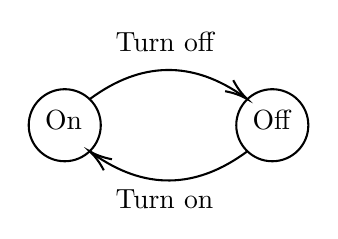
\begin{tikzpicture}[x=0.75pt,y=0.75pt,yscale=-1,xscale=1]
%uncomment if require: \path (0,199); %set diagram left start at 0, and has height of 199


% Text Node
\draw    (133, 145.5) circle [x radius= 17.36, y radius= 17.36]   ;
\draw (122,137) node [anchor=north west][inner sep=0.75pt]   [align=left] {On};
% Text Node
\draw    (233, 145.5) circle [x radius= 17.36, y radius= 17.36]   ;
\draw (222,137) node [anchor=north west][inner sep=0.75pt]   [align=left] {Off};
% Text Node
\draw (156,99) node [anchor=north west][inner sep=0.75pt]   [align=left] {Turn off};
% Text Node
\draw (156,175) node [anchor=north west][inner sep=0.75pt]   [align=left] {Turn on};
% Connection
\draw    (145,132.96) .. controls (169.82,114.56) and (194.66,114.19) .. (219.48,131.85) ;
\draw [shift={(221,132.96)}, rotate = 216.55] [color={rgb, 255:red, 0; green, 0; blue, 0 }  ][line width=0.75]    (10.93,-3.29) .. controls (6.95,-1.4) and (3.31,-0.3) .. (0,0) .. controls (3.31,0.3) and (6.95,1.4) .. (10.93,3.29)   ;
% Connection
\draw    (221,158.04) .. controls (196.18,176.44) and (171.34,176.81) .. (146.52,159.15) ;
\draw [shift={(145,158.04)}, rotate = 396.55] [color={rgb, 255:red, 0; green, 0; blue, 0 }  ][line width=0.75]    (10.93,-3.29) .. controls (6.95,-1.4) and (3.31,-0.3) .. (0,0) .. controls (3.31,0.3) and (6.95,1.4) .. (10.93,3.29)   ;

\end{tikzpicture}

    \caption{Light bulb FSM}
    \label{fig:simple_FSM}
\end{figure}


